\documentclass[fleqn,10pt]{wlscirep}

% Packages
\usepackage{pifont}
\usepackage{amsfonts}
\usepackage{amsmath}
\usepackage{float}
% \usepackage[multiple]{footmisc}
\usepackage{booktabs}
\usepackage{csquotes}
\usepackage{moreverb} % for verbatim ouput (for wordcount)
\usepackage{listings, textcomp}
\lstset{language=Python}

\lstset{ %
  basicstyle=\ttfamily\footnotesize,  % size of fonts used for the code
  breaklines=true,   % automatic line breaking only at whitespace
  captionpos=b,   % sets the caption-position to bottom
  commentstyle=\color{gray},  % comment style
  keywordstyle=\color{blue},  % keyword style
  stringstyle=\color{red},  % string literal style
  upquote=true  %straight single quotes (requires textcomp)
}

% New Commands
\newcommand{\cmark}{\ding{51}}%
\newcommand{\xmark}{\ding{55}}%
\newcommand{\code}[1]{\texttt{#1}}
\newcommand{\fixme}[1]{\textcolor{red}{{#1}}}
\newcommand{\inlinecite}[1]{\footnotesize\citen{#1}}
\newcommand{\tightlist}{\setlength{\itemsep}{0pt}\setlength{\parskip}{0pt}}


\usepackage{etoolbox}
\makeatletter
\patchcmd{\@maketitle}
 {\noindent
{\parbox{\dimexpr\linewidth-2\fboxsep\relax}{\color{color1}\large\sffamily\textbf{ABSTRACT}}}}
 {\noindent
{\parbox{\dimexpr\linewidth-2\fboxsep\relax}{\color{color1}\large\sffamily\textbf{ABSTRACT}}}}
 {}{}
\makeatother

\usepackage{lineno}
\linenumbers

\title{NumPy---Array Computation for Python}

\author[1]{Charles R. Harris}
\author[2,3,4,*]{K. Jarrod Millman}
\author[5,2,4,*]{St\'efan J. van der Walt}
\author[6,*]{Ralf Gommers}
\author[7]{Pauli Virtanen}
\author[8]{David Cournapeau}
\author[9]{Eric Wieser}
\author[10]{Julian Taylor}
\author[4]{Sebastian Berg}
\author[11]{Nathaniel J. Smith}
\author[12]{Robert Kern}
\author[4]{Matti Picus}
\author[13]{Stephan Hoyer}
\author[14]{Marten H. van Kerkwijk}
\author[2,15]{Matthew Brett}
\author[16]{Allan Haldane}
\author[17]{Jaime Fern\'andez del R\'io}
\author[18,19]{Mark Wiebe}
\author[6,20,21]{Pearu Peterson}
\author[22,23]{Pierre G\'erard-Marchant}
\author[24]{Kevin Sheppard}
\author[25]{Tyler Reddy}
\author[4]{Warren Weckesser}
\author[6]{Hameer Abbasi}
\author[26]{Christoph Gohlke}
\author[6]{Travis E. Oliphant}
\affil[1]{Independent Researcher, Logan, Utah, USA}
\affil[2]{Helen Wills Neuroscience Institute, University of California, Berkeley, Berkeley, CA, USA}
\affil[3]{Division of Biostatistics, University of California, Berkeley, Berkeley, CA, USA}
\affil[4]{Berkeley Institute for Data Science, University of California, Berkeley, Berkeley, CA, USA}
\affil[5]{Applied Mathematics, Stellenbosch University, Stellenbosch, South Africa}
\affil[6]{Quansight LLC, Austin, TX, USA}
\affil[7]{Department of Physics and Nanoscience Center, University of Jyv\"askyl\"a, Jyv\"askyl\"a, Finland}
\affil[8]{Mercari JP, Tokyo, Japan}
\affil[9]{Department of Engineering, University of Cambridge, Cambridge, UK}
\affil[10]{Independent Researcher, Karlsruhe, Germany}
\affil[11]{Independent Researcher, Berkeley, CA, USA}
\affil[12]{Enthought, Inc., Austin, TX, USA}
\affil[13]{Google Research, Mountain View, CA, USA}
\affil[14]{Department of Astronomy \& Astrophysics, University of Toronto, Toronto, ON, Canada}
\affil[15]{School of Psychology, University of Birmingham, Edgbaston, Birmigham, UK}
\affil[16]{Department of Physics, Temple University, Philadelphia, PA, USA}
\affil[17]{Google, Zurich, Switzerland}
\affil[18]{Department of Physics and Astronomy, The University of British Columbia, Vancouver, BC, Canada}
\affil[19]{Amazon, Seattle, Washington, USA}
\affil[20]{Independent Researcher, Saue, Estonia}
\affil[21]{Department of Mechanics and Applied Mathematics, Institute of Cybernetics at Tallinn Technical University, Tallinn, Estonia}
\affil[22]{Department of Biological and Agricultural Engineering, University of Georgia, Athens, GA}
\affil[23]{France-IX Services, Paris, France}
\affil[24]{Department of Economics, University of Oxford, Oxford, UK}
\affil[25]{CCS-7, Los Alamos National Laboratory, Los Alamos, NM, USA}
\affil[26]{Laboratory for Fluorescence Dynamics, Biomedical Engineering Department, University of California, Irvine, Irvine, CA, USA}
\affil[*]{millman@berkeley.edu, stefanv@berkeley.edu, ralf.gommers@gmail.com}


\keywords{Scientific computing, Python, Mathematics}

\begin{abstract}
  NumPy is the fundamental array computing library for Python.
  It has been actively developed for over two decades and has
  more than 850 contributors, nearly 300,000 dependent repositories
  on GitHub, and millions of downloads per year.
  It is extensively used in research and teaching.
  According to a 2018 survey, NumPy is the second most commonly used machine
  learning tool among enterprises \cite{451report2018}.
  In this article, we provide an overview of the capabilities and development
  practices of the NumPy library and highlight some recent technical
  developments.
\end{abstract}


\begin{document}

\flushbottom
\maketitle
\thispagestyle{empty}

% Count of words
\verbatiminput{wordcount.tex}

\section*{Introduction}

NumPy is the fundamental array computation library for the Python
ecosystem \cite{dubois2007guest,oliphant2007python,millman2011python,perez2011python}.
It underpins almost every library that does numerical
computation, including SciPy.  NumPy consists of the `ndarray`-object
along with utility functions to operate on such arrays.  Because of
its inherent simplicity—being a pointer to memory with some
associated meta-data about shape, data-type, and so forth—the NumPy
array has become the {\it de facto} exchange format for array data in
Python.  That said, NumPy has now seen such widespread adoption that
not only the array object but also its {\it Application Programming
  Interface} (API) has become ubiquitous, and is imitated by, e.g.,
popular tensor computation libraries.

Over the past few years, with external financial support, NumPy has
seen renewed developer interest.  It is actively developed to meet the
needs of its community, including the addition of some fairly significant
changes as outlined in the Recent technical improvements section below.

\subsection*{History}

NumPy was, at its inception, the unifier of the Python array
processing world.  Before NumPy, two packages—Numeric and
numarray—existed.  The first was developed by Jim Fulton, Jim Hugunin, Paul Dubois, Konrad
Hinsen, Travis Oliphant, and others, and was aimed at fast manipulation of many
small arrays.  In contrast, to handle large astronomical images,
NumArray was developed at the Space Telescope Science Institute (STScI).
In other words, these array
objects had different strengths and weaknesses, and therefore tended
to divide the already small user community.  In 2005, Travis Oliphant
started NumPy, a ``best of both worlds'' unification of the two
projects, based on Numeric.  The arrival of stable version 1.0 in October
2006 unified the scientific Python
community, and heralded the era of popular scientific computing in
Python that has led to formidable successes such as [cite some impacts here].

While, by 2006, NumPy was already eminently usable, it lacked good
documentation. In order to use NumPy in his classes, Joe Harrington
from the University of South Florida sponsored several rounds of the
NumPy Documentation Marathon \cite{harrington2008scipy,vanderwalt2008scipy}.
During these intensive
documentation improvement sessions, a Wikipedia-like system was
developed to allow community members to contribute so-called
``docstrings''—text describing each NumPy function. A community
documentation standard was published so that these pieces of
documentation would all provide similar information, and conform to a
basic standard of quality. Experienced community members reviewed and
integrated contributed docstrings, and soon NumPy had thorough
documentation coverage.

For a more detailed history of the scientific Python ecosystem, please
refer to ``SciPy 1.0---Fundamental Algorithms for Scientific Computing
in Python'' \cite{virtanen2019scipy}.

\subsection*{Funding}

For many years, NumPy operated without external funding, development
time mostly being contributed freely by students and researchers in
their spare time.  In-person meetings were sponsored off of
individual's research grants, and while industry sponsored
contributions were made, notably those by Mark Wiebe when he was
sponsored by Travis Oliphant at Continuum Analytics, mostly the package had rapid growth
and adoption without external investment.

% In 2014, NumPy received its
% first large grants from the Moore and Sloan foundations, totaling 1.3M
% dollars.  This allowed for hiring several full time programmers and,
% with the support of community members, mobilized a project that had
% become stagnant for the several years prior.

% BIDS -- UCB
% https://www.moore.org/grant-detail?grantId=GBMF5447
% $645,020 in 2016
% https://sloan.org/grant-detail/8222
% $659,359 in 2017
% https://bids.berkeley.edu/news/bids-receives-sloan-foundation-grant-contribute-numpy-development

The Berkeley Institute for Data Science (BIDS) received two grants to support
the development of NumPy.
At the end of 2016, the Gordon and Betty Moore Foundation awarded them
\$645,020 for improving NumPy for better data science.
In 2017, the Alfred P. Sloan Foundation complemented the funding with an
additional \$659,359.
Stéfan van der Walt, a senior research data scientist at BIDS and a member of
the NumPy steering committee, is the PI of both grants and manages a team of
four programmers working on the project.


% how much do we say about who these developers are and
% lessons learned?

% technical focus 
% improve various aspects of NumPy, including easier construction of custom data types (e.g., missing values, physical units, times & dates) and better integration with arrays customized for specialized domains (e.g., SciPy's sparse arrays, pandas' DataFrames, and xarray's labeled arrays). 
% technical work, and it increased the velocity of the projects by ~25-30%, and in addition it enabled integrating some larger changes, like the numpy.random redesign.

% CZI -- NumFOCUS/QuanSight
% https://chanzuckerberg.com/eoss/proposals/strengthening-numpys-foundations-growing-beyond-code/
% NumPy and OpenBLAS received $195,000 in 2019
% https://labs.quansight.org/blog/2019/11/numpy-openblas-CZI-grant/

NumFOCUS received a grant for \$195,000 in 2019 for the development of NumPy
and OpenBLAS from the Chan Zuckerberg Initiative. 
NumPy depends on OpenBLAS to provide its underlying accelerated linear algebra implementation.
Ralf Gommers, the Director of Quansight Labs and a member of
the NumPy steering committee, is the PI.

% focus on better serve NumPy's large number of beginner to intermediate level users
% focusing all our time on growing the team and better serving new users and contributors

% Tidelift, ...
% https://tidelift.com/subscription/pkg/pypi-numpy
% $10,000 over 24 months according to 
% https://mail.python.org/pipermail/numpy-discussion/2018-September/078736.html

% Intel, QuanSight, ...

\subsection*{Current status}

NumPy is now actively developed, with weekly online developer
meetings, a formalized NumPy enhancement proposal process, and
multiple active grants (but still almost no industry support).
% check almost no industry

% (maturity, users)

% \subsubsection*{Project goals / scope of library}

% https://numpy.org/neps/scope.html

% \subsubsection*{NEPS revived and roadmap}

Following Python's practice of using Python Enhancement Proposals (PEPs) for
``proposing major new features, for collecting community input on an
issue, and for documenting the design decisions that have gone into Python,''
we began using NumPy Enhancement Proposals (NEPs) in 2007.
This process was informal and only occasionally used until 2017 when
we adopted a more formal process \footnote{\url{https://numpy.org/neps/nep-0000.html}}.
Since then there have been 19 proposed NEPS---6 have been implemented,
4 have been accepted and are being implemented, 4 are under consideration,
3 have deferred or superseded, and 2 have been rejected or withdrawn.
We highlight a few of the implemented NEPs below.

% https://numpy.org/neps/roadmap.html


NumPy, while having been wildly successful as a library and array exchange
project, has now also become a standard language for expressing array and
tensor computations.  


\section*{Library organization}

Broadly, the NumPy library consists of the following parts:
the NumPy array data structure; the so-called \emph{universal functions};
a set of library functions for manipulating arrays and doing scientific
computation; infrastructure libraries for unit tests and Python package
building; and the program \code{f2py} for wrapping Fortran code in Python \cite{peterson2009f2py}.
The \code{ndarray} and the universal functions are generally considered
the core of the library.
In the following, we give a brief summary of these components of the
library.

\subsection*{Core.}

The \code{ndarray} data structure and the universal functions make up the core
of NumPy.

The \code{ndarray} is the data structure at the heart of NumPy.
The data structure stores regularly strided homogeneous data types
in a contiguous block memory, allowing for the efficient representation
of $n$-dimensional data.
More details about the data structure are given in ``The NumPy array:
a structure for efficient numerical computation.''\cite{vanderwalt2011numpy}.

The \emph{universal functions}, or more concisely, \emph{ufuncs},
are functions written in C that implement efficient looping over
NumPy arrays. An important feature of ufuncs is the built-in
implementation of \emph{broadcasting}.  For example, the function
\code{arctan2(x, y)} is a ufunc that accepts two values and computes
$\tan^{-1}(y/x)$.  When arrays are passed in as the arguments,
the ufunc will take care of looping over the dimensions of the inputs
in such a way that if, say, \code{x} is a 1-d array with length 3, and
\code{y} is a 2-d array with shape $2 \times 1$, the output will be
an array with shape $2 \times 3$.  The ufunc machinery takes care
of calling the function with all the appropriate combinations of
input array elements to complete the output array.
The elementary arithmetic operations of addition, multiplication, etc.,
are implemented as ufuncs, so broadcasting applies even in expressions
such as \code{x + y * z}.

\subsection*{Computing libraries}

NumPy provides a large library of functions for array manipulation
and scientific computing, including functions for: creating, reshaping,
concatenating, and padding arrays; searching, sorting and counting data
in arrays; computing elementary statistics, such as the mean, median,
variance, and standard deviation; file I/O; and more.

A suite of functions for computing the \emph{fast Fourier transform (FFT)}
and its inverse is provided.

NumPy's linear algebra library includes functions for: solving linear
systems of equations; computing various functions of a matrix, including
the determinant, the norm, the inverse, and the pseudo-inverse;
computing the Cholesky, eigenvalue, and singular value decompositions of a matrix;
and more.

The random number generator library in NumPy provides several alternative
\emph{bit stream generators} that provide the core function of generating
random integers.
A higher-level generator class that implements an assortment of
probability distributions is provided. It includes the beta, gamma
and Weibull distributions, the univariate and multivariate normal
distributions, and more.

A \emph{masked array} class, built on top of the \code{ndarray}, is
provided.  This class allows elements of an array to be masked,
indicating that the data is missing or unknown.

There is also a \code{matrix} class the implements 2-d arrays with
specialized behavior.  We mention it here for completeness, but the
use of \code{matrix} is discouraged.  The quirks of the \code{matrix}
class have proven to be troublesome, and with the addition of the
infix \code{@} operator to Python for matrix multiplication, there was no
longer a need for a separate \code{matrix} class, since one can
use a 2-d array instead.

\subsection*{Infrastructure libraries}

NumPy provides utilities for writing unit tests and for building Python
packages.

The \code{testing} subpackage provides functions such as
\code{assert\_allclose(actual, desired)} that may be used in unit
test suites for code that uses NumPy arrays.

NumPy provides a subpackage includes functions and classes
that can be used by libraries that have NumPy as dependency,
to be used in the library's configuration code that installs the
library and that builds a package that can be used, for example,
on the PyPI web site.

The program \code{f2py} is a tool for
building NumPy-aware Python wrappers of Fortran functions.
NumPy itself does not use any Fortran code;  F2PY is part of NumPy
for historical reasons.

\section*{Common infrastructure}

In addition to the testing and building packages described above,
as the fundamental package for numerical and scientific computing
in Python, NumPy also plays a central role in building and
standardizing much of the community infrastructure.
The docstring standard mentioned in the history section is now
widely adopted.

% https://numpy.org/neps/nep-0029-deprecation_policy.html
In NEP 29, we recommend, along with leaders from various other
projects, that all projects across the Scientific Python ecosystem
adopt a common ``time window-based'' policy for support of Python and
NumPy versions. This standard will simplify downstream project and
release planning.

\subsection*{Wheels build system}

A Python \emph{wheel}\cite{PEP427} is a standard file format for
distributing Python libraries.  In addition to Python code, a
wheel may include compiled C extensions and other binary data.
This is important, because many libraries, including NumPy,
require a C compiler and other build tools to build the software
from the source code, making it difficult for many users to install
the software on their own.  The introduction of wheels to the Python
packaging system has made it much easier for users to install
precompiled libraries.

A GitHub repository containing scripts to build NumPy wheels has
been configured so that a simple commit to the repository triggers
an automated build system that creates NumPy wheels for several
computer platforms, including Windows, Mac OSX and Linux.  The wheels
are uploaded to a public server and made available for anyone to use.
This system makes it easy for users to install precompiled versions
of NumPy on these platforms.

The technology that is used to build the wheels evolves continually.
At the time this paper is being written, a key component is the
\code{multibuild} suite of tools developed by Matthew Brett and
other developers\cite{multibuild}.  Currently, scripts using
\code{multibuild} are written for the continuous integration
platforms Travis-CI (for Linux and Mac OSX) and Appveyor
(for Windows).


\section*{Recent technical improvements}

\subsection*{Random}

The NumPy random module provides pseudorandom numbers from a wide range of
distributions. In legacy versions of NumPy, simulated random values are produced
by a \code{RandomState} object that: handles seeding and state initialization;
wraps the core pseudorandom number generator based on a 32-bit implementation of
MT19937; interfaces with the underlying code that transforms random bits into
deviates from other distributions; and supplies a singleton instance exposed in
the root of the random module.

The \code{RandomState} object makes a compatibility guarantee so that a fixed
seed and sequence of function calls produce the same set of values. This
guarantee has slowed progress since improving the underlying code requires
extending the API with additional keyword arguments. This guarantee continues to
apply to \code{RandomState}. 

NumPy 1.17 introduced a new API for generating random numbers that use a more
flexible structure that can be extended by libraries or end-users. The new API
is built using components that separate the steps required to generate random
variates. Pseudorandom bits are generated by a bit generator. These bits are
then transformed into variates from complex distributions by a generator.
Finally, seeding is handled by an object that produces sequences of high-quality
initial values.

Bit generators are simple classes that manage the state of an underlying
pseudorandom number generator. NumPy ships with four bit generators. The default
bit generator is a 64-bit implementation of the Permuted Congruential Generator
\cite{pcg64} (\code{PCG64}). The three other bit generators are a 64-bit version
of the Philox generator\cite{random123} (\code{Philox}), Chris Doty-Humphrey's
Small Fast Chaotic generator\cite{practrand} (\code{SFC64}), and the 32-bit
Mersenne Twister\cite{mt19937} (\code{MT19937}) which has been used in older
versions of NumPy.\footnote{The
\href{https://github.com/bashtage/randomgen}{randomgen project} supplies a wide
range of alternative bit generators such as a cryptographic counter-based
generators (\code{AESCtr}) and generators that expose hardware random number
generators (\code{RDRAND})\cite{randomgen}.} Bit generators export a capsule
containing pointers to functions that produce 64 bits, 32 bits, or a random
double. They also expose CFFI and ctypes interfaces to the same three functions.

The \code{Generator} consumes one of the bit generators and produces variates
from complicated distributions. Many improved methods for generating random
variates from common distributions were implemented, including the Ziggurat
method for normal, exponential and gamma variates\cite{ziggurat}, and Lemire's
method for bounded random integer generation\cite{lemire}. The \code{Generator}
is more similar to the legacy \code{RandomState}, and its API is substantially
the same. The key differences all relate to state management, which has been
delegated to the bit generator. The \code{Generator} does not make the same
stream guarantee as the \code{RandomState} object, and so variates may differ
across versions as improved generation algorithms are
introduced.\footnote{Despite the removal of the compatibility guarantee, simple
reproducibility across versions is encouraged, and minor changes that do not
produce meaningful performance gains or fix underlying bug are not generally
adopted.}

Finally, a \code{SeedSequence} is used to initialize a bit generator. The seed
sequence can be initialized with no arguments, in which case it reads entropy
from a system-dependent provider, or with a user-provided seed. The seed
sequence then transforms the initial set of entropy into a sequence of
high-quality pseudorandom integers, which can be used to initialize multiple bit
generators deterministically. A key design goal of a seed sequence was to be
splittable in the sense that a seed sequence can be used to produce child
sequences that are distinct from their parents or other ancestors. This
capability allows a seed sequence to be used in large distributed applications
where the number of workers required is not known. The sequences generated from
the same initial entropy and the same splits are fully deterministic to ensure
reproducibility.

The three components are combined to construct a complete random number
generator.

\begin{lstlisting}
from numpy.random import Generator, PCG64, SeedSequence
seq = SeedSequence(10304245474441179933310169597522947680)
pcg = PCG64(seq)
gen = Generator(pcg)
\end{lstlisting}

\noindent This approach retains access to the seed sequence which can then be
used to spawn additional generators.

\begin{lstlisting}
children = seq.spawn(2)
gen_0 = Generator(PCG64(children[0]))
gen_1 = Generator(PCG64(children[1]))
\end{lstlisting}

\noindent While this approach retains complete flexibility, the method
\code{np.random.default\_rng} can be used to instantiate a \code{Generator} when
reproducibility is not needed.

The final goal of the new API is to improve extensibility. \code{RandomState} is
a monolithic object that obscures all of the underlying state and functions. The
component architecture is one part of the extensibility improvements. The
underlying functions (written in C) which transform the output of a bit
generator to other distributions are available for use in CFFI. This allows the
same code to be run in both NumPy and dependent that can consume CFFI, e.g.,
numba. Both the bit generators and the low-level functions can also be used in C
or Cython code.\footnote{As of 1.18.0, this scenario requires access to the
NumPy source. Alternative approaches that avoid this extra step are being
explored.} 

\subsection*{The Array Function Protocol}

The central position which NumPy takes within the numerical and scientific
Python ecosystem  means that a vast number of projects are built on it.
These projects are consumers of the NumPy API.

On the other side, projects are providers of a \emph{NumPy-like API} and array
objects targeting audiences with specialized needs beyond NumPy's capabilities.
For example, the NumPy API is implemented by
several popular tensor computation libraries including
CuPy\footnote{\url{https://cupy.chainer.org/}},
Jax\footnote{\url{https://jax.readthedocs.io/en/latest/jax.numpy.html}},
PyTorch\footnote{\url{https://pytorch.org/tutorials/beginner/blitz/tensor\_tutorial.html}}, and
Apache MXNet\footnote{\url{https://mxnet.incubator.apache.org/api/python/docs/api/ndarray/index.html}},
and to a lesser extent
TensorFlow\footnote{\url{https://www.tensorflow.org/api\_docs/python/tf/Tensor}}.
It is also implemented in packages that support sparse arrays
such as \code{scipy.sparse} and \code{pydata.sparse}.
Another notable example is Dask, a library for parallel computing in
Python.  Dask adopts the NumPy API and therefore presents a familiar
interface to existing NumPy users, while adding powerful abilities to
parallelize and distribute tasks.

The multitude of specialized projects creates the difficulty that consumers
of these NumPy-like APIs write code specific to a single project and do not support
all of the above array providers.
This is a burden for users relying on the specialized Array-like, since
a tool they need may not work for them.
Additionally, a user who has the need of transitioning from NumPy to a more
specialized array, is faced with a challenge.
These issue can lead into a fragmentation of the user bases into consumers
of different NumPy-like APIs.

To address these issues NumPy has the goal of providing the fundamental
API for \emph{interoperability} between the various NumPy-like APIs.
An earlier step in this direction was the implementation of the
\code{\_\_array\_ufunc\_\_} protocol in NumPy 1.13, which enabled interoperability
for most mathematical functions.\cite{NEP13}
In 2019 this was expanded more generally with the inclusion of the
\code{\_\_array\_function\_\_} protocol into NumPy~1.17.
These two protocols allows providers of Array-like APIs to be interoperable
with the NumPy API: their arrays work correctly with almost all NumPy functions.\cite{NEP18}
For the users relying on specialized array projects it means that even though
much code is written specifically for NumPy arrays and uses the NumPy API as
\code{import numpy as np}, it can nevertheless work for them.
A brief example of such a function which is written using NumPy
but can now be used more generally is:
\begin{lstlisting}
def f(x):
    y = np.tensordot(x, x.T)
    return np.mean(np.exp(y))
\end{lstlisting}
For example, a user relying on this function and normally using it with a
NumPy array, may now use a distributed Dask array when challenged
by a very large dataset, without any modification to \code{f(x)}.

%In order to aid better interaction between NumPy and these libraries,
%an ``array function'' protocol was added to NumPy in 2018 (see Section
%X). The new protocol allows for external array objects (sometimes
%called ``duck arrays'') to pass through NumPy:
%
%\begin{lstlisting}
%  import numpy as np
%  import cupy as cp
%
%  x_gpu = cp.array([1, 2, 3])
%  y = np.sum(x_gpu)  # This works, and returns a GPU array
%\end{lstlisting}


\subsection*{Testing on multiple architectures}

At the time of writing the two fastest supercomputers in the
world, Summit and Sierra, both have IBM POWER9 architectures
\cite{top500nov2019}. In late 2018, Astra, the first ARM-based
supercomputer to enter the TOP500 list, went into production\cite{
astra-wiki}. Furthermore, over 100 billion ARM processors have been
produced as of 2017\cite{arm-architecture}, making it the most 
widely used instruction set architecture in the world.

Clearly there are motivations for a large scientific computing
software library to support POWER and ARM architectures. We've extended
our continuous integration (CI) testing to include \texttt{ppc64le}
(POWER8 on Travis CI) and ARMv8 (on Shippable service). We also test
with the s390x architecture (IBM Z CPUs on Travis CI) so that we
can probe the behavior of our library on a big-endian machine.
This satisfies one of the major components of
improved CI testing laid out in a version of our roadmap
\cite{numpy-roadmap}---specifically, ``CI for more exotic
platforms."

PEP 599\cite{PEP599} lays out a plan for new Python binary wheel
distribution support, \texttt{manylinux2014}, that adds
support for a number of architectures supported by the CentOS
Alternative Architecture Special Interest Group, including
ARMv8, ppc64le, as well as s390x. We are thus well-positioned
for a future where provision of binaries on these architectures
will be expected for a library at the base of the ecosystem.

\section*{Project organization and community}

\subsection*{Governance}

% incl. CoC

\subsection*{Maintainers and contributors}

%  nr of core devs / commit rights) & contributors

NumPy is currently maintained a group of 23 contributors with commit rights
to the NumPy code base. Out of these 17 maintainers were active in 2019.
Additionally, there are a few long term developers who contributed and maintain
specific parts of NumPy, but are not officially maintainers.
At a release cycle of about every half year, the five recent releases in the years
2018 and 2019 have averaged about 450~pull requests~(PR) each.\footnote{
    Note that before mid 2011, NumPy development did not happen on \url{github.com}.
    All data provided here is based on the development which happened through github
    pull requests. In some cases contributions by maintainers may not be categorized as such.}
% Since 1.14.0 (based on changelog): 381 + 438 + 490 + 531 + 402; last is preliminary
With each release attracting more than a hundred new contributors.

\begin{figure}
    \centering
    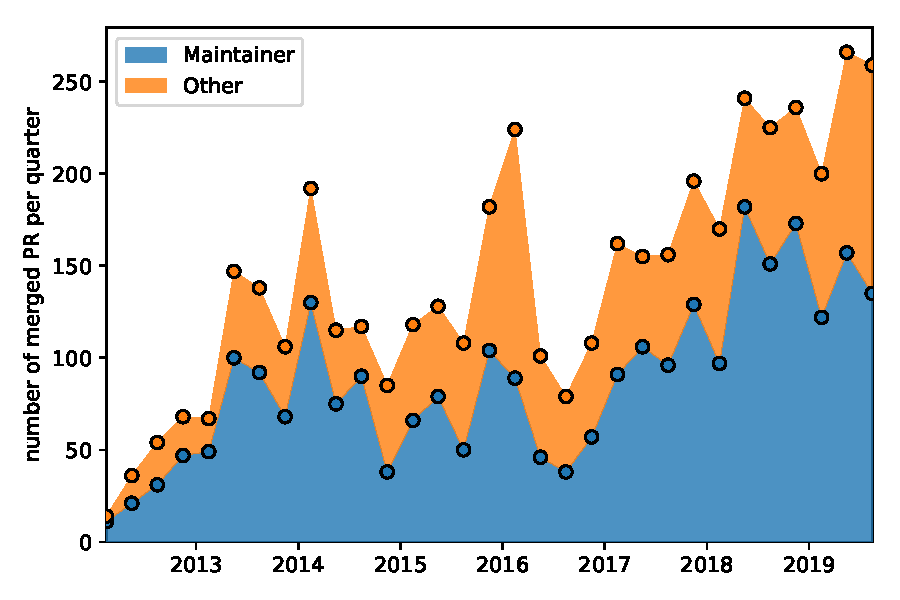
\includegraphics[width=0.5\textwidth]{scripts/PRs-using-CURRENT_MAINTAINERS.pdf}
    \caption{Number of pull requests merged into the NumPy master branch for each
        quarter since 2012. The total number of PR is indicated with the
        lower blue area showing the portion contributed by current or previous
        maintainers.}\label{fig:prs-over-time}
\end{figure}

The stacked plot in Figure~\ref{fig:prs-over-time} shows the number of
PR merged into the NumPy master branch.
In this plot PR opened by current and old maintainers are indicated.
Although the number of PRs being merged fluctuates,
the plot indicates an increased number of contributions over the past
years.
Over the course of its history, NumPy has attracted PR by 823 contributors.
However, its development still relies heavily on the relative small number
of stable maintainers, who share more than half of the contributions among
themselves.


% may be useful:
% - https://github.com/docathon/watchtower
% - https://github.com/machine-shop/oss_devkit/blob/master/plot_pr.py % (PR over time plot, there may be other better versions out there)

% \subsection*{GSoD}


\section*{Discussion}

Most of the technical work for the Moore and Sloan grant is now complete.
The main remaining item is an overhaul of the data type system, which is discussed
below.  Now that years of technical debt have been addressed, the project
is in good shape for growing the community and better addressing the needs
of new users.  That is the main focus of the CZI grant, which we discuss
below.

% \subsubsection*{Future Development}

% Dtypes

The meaning of each element within a NumPy array is described by its datatype
(dtype). NumPy arrays can hold all common numerical datatypes, string, datetimes
and generic Python objects, each of these is identified by a dtype.
We are busy overhauling the datatype system to make it consistent (aligned with
expectations), to simplify the creation of custom dtypes.
While numerical dtypes make the foundation for most users, there are
a multitude of use cases which cannot prosper due to current limitations.
These use cases include datatypes with physical units\cite{astropy,Goldbaum2018,pint},
% pyadolc may be a bit too small a project, so may want to remove/replace with an other example.
geometrical objects\cite{pygeos}, automatic differentiation\cite{pyadolc}, and many more.
Projects addressing these exist, each struggles with current
limitations.  % TODO: I may need citations, we could link github issues.

While it is currently possible to define custom dtypes within NumPy, many of the
use cases above cannot be solved using this system.
This is evidenced also by code within NumPy which would require changes
in many places to add such dtypes, even when adding them within NumPy itself.
The new implementation will be simpler and more cleanly implemented in
this regard.
Custom dtypes and the basic dtypes included within NumPy will be implemented
and behave identically as much as possible.
At the same time redesigning the API will make NumPy dtypes more flexible to grow
to future needs should they arise.

As a further step, to make dtypes more accessible and allow a faster adoption of
custom dtypes within the community, we plan to create a Python API to
define such custom dtypes.

A \href{https://github.com/numpy/numpy/pull/14422}{draft of DTypes NEP}
is under development in consultation with the community.

% outline plan for the CZI grant and an invitation to new contributors

%\subsection*{Website}

\section*{Data Availability}

All NumPy source code and most data generated for the current study are
available in the NumPy GitHub repository, \url{https://github.com/numpy}. Some
supporting code and data have also been stored in other public repositories
cited by this manuscript.

\bibliography{references}

\section*{Acknowledgments}


\section*{Author Contributions Statement}

%Must include all authors, identified by initials, for example: A.A.
%conceived the experiment(s),  A.A. and B.A. conducted the experiment(s), C.A.
%and D.A. analysed the results.  All authors reviewed the manuscript.

\section*{Competing Interests}

The authors declare no competing interests.

\section*{Consortium}
\subsection*{NumPy Contributors}

{\bfseries
Adam Apple$^{5}$
}
\newline
\hfill \break
$^{5}$International Centre for Ecological Exploration, California, USA


\end{document}

%%% Local Variables:
%%% mode: latex
%%% TeX-master: t
%%% End:
